% -*- mode: LaTeX; coding: utf-8; -*-

\chapter{Tiedon keruu ja esikäsittely}

Luvussa \ref{sec:lahtokohta} kuvailtiin tutkittavien lokitiedostojen
alkuperää ja tiedostomuotoa. Tässä luvussa tutustutaan
seikkaperäisemmin siihen, miten Ixonokselta saamamme palvelinloki on
järjestetty tiedostoihin ja millä tavoin tietoa on esikäsitelty
analyysiä silmällä pitäen. Käytetyt menetelmät soveltuvat pienin
muutoksin myös muiden Web-hotellien palvelinlokien esikäsittelyyn,
mikäli arkistointikäytänteet eivät suuresti poikkea tässä esitellystä.

Esimerkeissä käytetyt palvelinten ja palveluiden nimet ovat
kuvitteellisia, mutta rakenne vastaa tutkittua ympäristöä.

 % - Mistä data on peräisin?
 %    - Palvelun rakenteen kuvaus
 % - Millaista data on?
 %   - HTTP
 %   - Apachen logit
 % - Miten data on kerätty? (ohjelmistot ja verkkotopologia)
 %   - Yleisellä tasolla
 % - Mitä työkaluja on käytetty (Haskell ja PhasefulSplitter)
 % - Miten dataa on käsiteltu ja suodatettu?

\section{Tiedon rakenne}

Ixonoksen Web-hotelli on toteutettu siten, että yksittäiset palvelut on
sijoitettu jokaiselle palvelimelle. Ratkaisun taustalla on
kuormituksen tasaaminen. Erillinen järjestelmä huolehtii siitä, että
Internetistä tulevat kyselyt ohjataan tasaisesti eri
palvelimille. 

Taulukossa \ref{nimet} on esimerkki palveluiden ja
palvelinten nimeämisestä.

% Ei kannata ottaa esimerkkiä tästä taulukosta, tämä on vähän mutkikas.
\begin{table}[h]
\centering
\begin{tabular}{lll}
Palvelin && Palvelu \\
\cline{1-1}\cline{3-3}
dapper && buzz \\
edgy && rex \\
feisty && potato \\
&& hamm \\
&& slink \\
\end{tabular}
\caption{Palvelinten ja palveluiden nimeäminen.}
\label{nimet}
\end{table}

Lokitiedostot on sijoitettu hakemistorakenteeseen, jossa juuressa ovat
palvelinten nimien mukaiset hakemistot, joiden sisällä sijaitsevat
lokitiedostot, jotka on nimetään yhdistämällä palvelun nimi
päivämääräleimaan. Tiedostonnimessä käytetty päivämäärän muoto
noudattaa ISO 8601 -standardia~\cite{iso8601}. Tiedostot on pakattu
\texttt{gzip}-pakkausohjelmalla. Taulukossa \ref{tiedostot}
havainnollistetaan tiedostonnimien muodostumista.

\begin{table}[h]
\centering
\begin{tabular}{llll}
Palvelin & Palvelu & Päivämäärä & Tiedostonnimi \\
\hline
edgy & buzz & 14.6.2009 & \texttt{edgy/buzz.http.2009-06-14.gz}\\ 
dapper & potato & 2.7.2009 & \texttt{dapper/potato.http.2009-07-02.gz}\\
feisty & rex & 30.7.2009 & \texttt{feisty/rex.http.2009-07-30.gz}\\
\end{tabular}
\caption{Tiedostojen nimeäminen.}
\label{tiedostot}
\end{table}

Tässä mainittujen palvelinten lisäksi käytössä on ulkoinen
välimuistipalvelu, jonka kautta välitetään harvoin muuttuvia
resursseja, kuten kuvia. Valtaosa dataliikenteestä
välitetään palvelun kautta. Välimuistipalvelu toimii siten, että
mikäli pyydettyä resurssia ei löydy sen omasta muistista, se pyytää
sitä yhdeltä Web-hotellin palvelimista ja välittää vastauksen edelleen
asiakkaalle. Välimuistipalvelun käyttö ei kuitenkaan muilta osin
vaikuta palvelun rakenteeseen. Rakenne käy ilmi kuvasta
\ref{palvelinrakenne}.

\begin{figure}[htp]
\centering
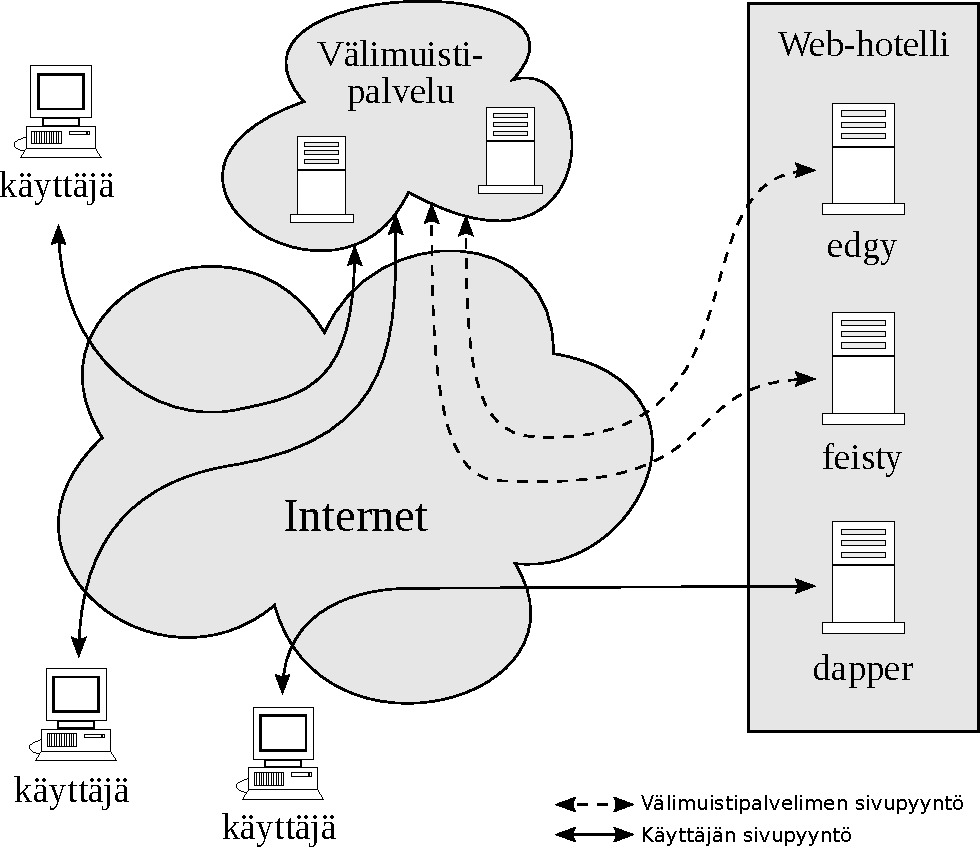
\includegraphics[width=12cm]{pics/palvelinrakenne.pdf}
\caption{Web-palvelun rakenne.}
\label{palvelinrakenne}
\end{figure}

\section{Esikäsittely}

\todo{Tästä puuttuu vielä tekstiä!}

Luvussa \ref{sec:lahtokohta} esiteltiin lokitiedostoissa käytetty
\textit{Combined Log Format} -muoto. Tiedosto on tekstimuotoinen,
joten se ei sellaisenaan sovellu analyysivaiheeseen, jossa käsitellään
klustereita. Osa palvelinlokin sisällöstä on myös analyysin kannalta
tarpeetonta ja nämä osat tulee suodattaa pois. Lisäksi yhteen
Web-palveluun liittyvät kyselyt ovat lisäksi jakautuneet useaan eri
tiedostoon eri palvelinten ja vuorokausien mukaisesti.

Esikäsittelijä on toteutettu osana tätä tutkimusta. Esikäsittelijä on
nimeltään \textit{PhasefulSplitter} ja se on toteutettu
Haskell-ohjelmointikielellä~\cite{haskell98}. Haskell tarjoaa
tehokkaat työkalut ohjelmakoodin rinnakkaistamiseen ja datan
sarjallistamiseen. \textit{PhasefulSplitter} on vapaa ohjelma ja sitä saa
levittää edelleen ja muuttaa Free Software Foundationin julkaiseman
GNU General Public Licensen (GPL-lisenssi) version 3~\cite{gplv3} tai (valinnan
mukaan) myöhemmän version ehtojen mukaisesti. Esikäsittelijä on
ladattavissa Internetistä osoitteesta \\
\url{http://iki.fi/zouppen/repo/phasefulsplitter.git}.

Esikäsittelijä on jaettu useaan itsenäiseen osaan, mikä helpottaa
datan käsittelyä jälkikäteen erilaisin menetelmin. Lisäksi
sarjallistetut tietorakenteet voidaan tarvittaessa anonymisoida,
jolloin dataa voidaan luovuttaa myös ulkopuoliseen käyttöön.

Esikäsittely jakaantuu seuraavaat kolmeen vaiheeseen:

\begin{enumerate}
\item Tiedostolistan muodostaminen ja tiedostojen ryhmittely palveluittain.
\item Tiedostojen sisällön lukeminen ja muuntaminen tietorakenteeksi.
\item Tietorakenteiden jatkokäsittely.
\end{enumerate}

\subsection{Tiedostolistan muodostaminen}

TODO

\subsection{Muuntaminen tietorakenteeksi}

Toisessa vaiheessa tekstimuotoiset lokitiedostot luetaan ja
käsitellään koneellisesti helpommin analysoitavaan
muotoon. Tätä työtä varten kehitetyssä tiedonkäsittelijässä
lokitiedoston eri kentät palastellaan ja kyselyt sarjallistetaan tiedostoihin.

TODO

\subsection{Jatkokäsittely}

Lopuksi eri kenttien numeeriset ja
luokka-asteikolliset arvot klusteroidaan.

TODO

\begin{comment}
Tiedostolistan luonti
---------------------

Tiedostolistan esikäsittely on täysin riippuvainen siitä, miten
logitiedostot on nimetty. Mitään suoraa ohjetta tähän on vaikea
antaa. Tässä käytetään ns. Ixonos-nimeämistä eli muotoa
'/polku/palvelimennimi/palvelunnimi.YYYY-MM-DD.gz'. Palvelut ovat
toisistaan irrallisia (ainakin analyysin mielekkyyden kannalta). Yksi
palvelu koostuu useammalla palvelimesta ja näillä oleva sisältö on
identtistä.

Luokittelussa tarvitaan palvelinten nimet. Ne asetetaan tiedostoon
'server.map' seuraavan esimerkin mukaisesti:

$ cp server_map.txt.example server_map.txt
$ emacs server_map.txt  # or nano, vim ...

Tehdään tiedostolista käyttämällä esimerkiksi findiä:

$ find /path/to/log -iname '*.gz' >tiedostolista.txt

Suoritetaan luokittelija, joka jakaa tiedostot eri palveluiden mukaan
ja tallentaa ne levylle hakemistoon 'lists'

$ mkdir lists
$ ./classifier tiedostolista.txt lists/

Voit myös antaa tiedostolistan syötteenä näin:

$ find ... | ./classifier lists/

Jakaminen binaaritiedostoihin
-----------------------------

xargs-komennolla voi nätisti ajaa rinnakkain eri ytimillä tiedostojen
esikäsittelyn ohjelman omaan .pf.gz -muotoon. Allaolevassa esimerkissä
esikäsitellään lists-hakemistosta löytyvät tiedostolistat ja
kirjoitetaan ne hakemiston data alle. Tiedostolistat esikäsitellään 8
ytimellä ja kirjoitetaan 8 eri tiedostoon kukin. Jako mahdollistaa
tehokkaan jälkikäsittelyn, koska tiedostojen sisältöä on mahdollista
käsitellä myöhemmin samanaikaisesti.

$ ls lists/*| xargs -n 1 -I{} -P 8 ./apache2data 8 {} data/

N-grammianalyysi
----------------

N-grammianalyysissä ensin kerätään tiedot niistä n-grammeista, jotka
esiintyvät datassa. ParameterAnalyzer.hs:ssä on kiinteästi määritelty
2-grammien laskeminen, mutta tätä vakiota voi helposti muuttaa.
N-grammien esiintyvyyskartan laatiminen on välttämätöntä muistin
säästämiseksi. Muutoin muodostuisi 256^n kokoinen vektori, kun
käsiteltävät merkkijonot koostuvat Word8-tyypeistä (8-bittinen tavu).

N-grammilistoja muodostuu yhtä paljon kuin on eri resurssien
get-parametreja. Tämä vaihtelee runsaasti eri Web-palveluissa.
Lopputulos on kuitenkin vain murto-osa alkuperäisen datamassan
suuruudesta.

Muodostetaan yhdelle palvelulle 2-grammit. Mene hakemistoon, jossa
palvelun datatiedostot ovat (eli sinne, josta löytyy mm. 1.pf.gz:

$ parameter_analyzer *.pf.gz +RTS -N

Hakemistoon muodostuu ajon seurauksena tiedostot 'ngrams.out' ja
'ngrams_raw.txt'. Näistä ensimmäinen on binaarimuodossa ja sisältää
datan jatkokäsittelyä varten. Toisessa tiedostossa on tekstimuodossa
(Haskellin show-muodossa) eri resurssien ja n-grammien
esiintymistiheydet. Sitä voi käyttää apuna selvittäessä, mitä
kannattaisi tuttkia. Tutkiminen kannattaa keskittää palveluihin,
joissa on runsaasti parametreja.

TODO
\end{comment}


\section{Analysoinnin vaiheet}

Kolmannessa vaiheessa tapahtuu varsinainen analysointi. Käytetty
anomalia-analyysi edellyttää, että aineiston muuttujat ovat
luokka-asteikollisia ja tästä johtuen tieto on klusteroitu edeltävässä vaiheessa.

\subsection{Tiedon keruu}

TODO.

\subsection{Esikäsittely}

Sopivaa yksivaiheista parseria käyttämällä olisi mahdollista käsitellä
lähtödata suoraan analyysissä käytettävään muotoon. Käytännössä kuitenkin datan
esikäsittely kannattaa hoitaa useammassa vaiheessa, jotta datassa
olevat puuttuvat tai poikkeavat arvot tulee huomioitua
asianmukaisesti. Monivaiheinen esikäsittely helpottaa myös saman
lähtödatan käyttämisen useaan eri analyysiin.

Tiedon käsittelyn helpottamiseksi tässä työssä käytetään esikäsittelyn
välivaiheiden ja lopputuloksen tallentamiseen
relaatiotietokantaa. Relaatiotietokanta mahdollistaa useiden
esikäsittelyn vaiheiden suorittamisen vähäisellä ohjelmoinnilla ja
helposti ymmärrettävästi.

Tässä työssä käsiteltävää aineistoa varten on kehitetty ``PhasefulSplitter
'' -sovellus esikäsittelyä varten.

TODO.

\subsection{Kategorisointi}

TODO.
